%
% 1_prinzip_1d.tex -- Das Prinzip der Methode der finiten Elemente in einer Dimension
%
% (c) 2024 Flurin Brechbühler, OST - Ostschweizer Fachhochschule Rapperswil
%
% !TEX root = ../../buch.tex
% !TEX encoding = UTF-8
%
\section{Prinzip 1D\label{fem:prinzip_1d}}
\kopfrechts{Prinzip 1D}

Das Vorgehen zum Herleiten der Metode der Finiten Elemente kann in sechs Schritte unterteilt werden:
\begin{itemize}
    \item Bilden der Schwachen Form
    \item Diskretisieren
    \item Aufstellen des linearen Gleichungssystems
    \item Überführung in eine Matrix
    \item Codieren der Anfangsbedingungen
    \item Lösen des Gleichungssystems bzw. invertieren der Matrix
\end{itemize}

Um die einzelnen Schritte darzustellen, betrachten wir das Problem
\begin{equation}
    u''(x) = f(x)
    \label{fem:1d:poisson_gleichung},
\end{equation}
was der Poisson-Gleichung entspricht. 
Diese findet in vielen Teilen der Physik Anwendung und ist gleichzeitig ein gutes, einfaches Beispiel einer mit der FEM lösbaren Differentialgleichung.


\subsection{Bilden der Schwachen Form\label{fem:1d:schwache_form}}
Um die Poisson-Gleichung in die Schwache Form zu bringen, wird über beide Seiten der Poisson-Gleichung \ref{fem:1d:poisson_gleichung} integriert.
Zufor werden jedoch beide Seiten mit der Testfunktion $ v(x) $ multipliziert. % TODO: Testfunktion -> Variation
Diese wird definiert als eine beliebige Funktion $ v: \mathbb{R} \rightarrow \mathbb{R} $.
Die resultierende Gleichung
\begin{equation}
    \int(u''(x) \cdot v(x) \diff x) = \int(f(x) \cdot v(x) \diff x) \myforall v(x)
    \label{fem:1d:schwache_form_equation}
\end{equation}
sollte einem bekannt vorkommen: Sie entsteht auch beim Herleiten der ersten Variation.
Im Kapitel \ref{buch:variation:fundamentallemma} zum Fundamentalemma wird bewiesen, dass die beiden Ausdrücke \ref{fem:1d:poisson_gleichung} und \ref{fem:1d:schwache_form} gleichwertig sind.

Durch partielles Integrieren der linken Seite kann die Ordnung der Differentialgleichung um eins verringert werden:
\begin{align}
    \int f(x) \cdot v(x) \diff x &= \int u''(x) \cdot v(x) \diff x \\
                                 &= \left. u'(x) \cdot v(x) \right|_{x_1}^{x_2} - \int u'(x) \cdot v'(x) \diff x \\
                                 &= - \int u'(x) \cdot v'(x) \diff x \\
                                 &= - \Phi(u, v)
\end{align}
wobei der Term
\begin{equation}
    \left. u'(x) \cdot v(x) \right|_{x_1}^{x_2}
\end{equation}
Null ist, wenn die Testfunktionen die Bedingung
\begin{equation}
    v(x_1) = v(x_2) = 0
\end{equation}
erfüllen. % TODO: Hat das nicht implikationen für das Setzen von Randbedingungen?

Der erhaltene Term wird als $-\Phi(u, v)$ abgekürzt.
Dieser Weg kann, abhängig von der ursprünglichen Differentialgleichung, anders sein.
Das häufigste Vorgehen dabei - das partielle Ableiten der rechten Seite - wurde jedoch hier gezeigt.
Ziel ist es, die Ordnung der Differentialgleichung möglichst stark zu verkleinern, da so Ansätze kleiner Ordnung verwendet werden können.
Dies spart Rechenleistung.


\subsection{Diskretisieren\label{fem:1d:diskretisieren}}
Um das Problem besser lösbar zu machen, werden die kontinuierlichen Funktionen als Summe einzelner Funktionen mit schmalem Träger 
\begin{equation}
    a(x) = \left\{ \begin{array} {ll}
        a(x) = 1            & \mbox{für} x = 0 \\
        a(x) \in \mathbb{R} & \mbox{für} 0 < |x| < \Delta t \\
        a(x) = 0            & \mbox{sonst} 
    \end{array}\right.
\end{equation}
beschrieben:
\begin{equation}
    u(x) \approx \sum{u_n \cdot a_n(x)} \mbox{ und } v(x) \approx \sum{v_n \cdot a_n(x)}
\end{equation}
wobei 
\begin{equation}
    u_n = u(n \cdot \Delta x) \mbox{ und } v_n = v(n \cdot \Delta x)
\end{equation}
sowie 
\begin{equation}
    a_n(x) = a(x - n \cdot \Delta x).
\end{equation}

Dabei wird die ursprüngliche Funktion an den gleichmässig verteilten Punkten $x_n = n \cdot \Delta x$ gesampelt. 
Die Funktion könnte auch ungleichmässig abgetastet werden, was bei geschickter Wahl der Intervalllänge zu Effizienzverbesserungen führt.
In diesem Paper werden, um die Erklärung möglichst einfach zu halten, nur gleichmässige Intervalle behandelt. 

Für die Interpolationsfunktion $a(x)$ können verschiedene Ansätze gewählt werden:
\begin{itemize}
    \item[\textbf{linear:}] 
        Einfach zu rechnen und zu verstehen, jedoch ist die erste Ableitung unstetig und die zweite Ableitung Null.
        Dementsprechend kann dieser Ansatz nur verwedet werden, wenn keine zweiten Ableitungen im vereinfachten Problem vorkommen.
    \item[\textbf{quadratisch:}]
        Ist die Ordnung des Problems um eins zu hoch, um den linearen Ansatz zu verwenden, kann der quadratische Ansatz eingesetzt werden.
        Die ersten Ableitungen sind jedoch nach wie vor unstetig.
    \item[\textbf{kubisch:}]  
        Der kubische Ansatz hat sehr gute Eigenschaften - er besitzt eine stetige erste Ableitung sowie zweite und dritte Ableitungen ungleich Null. 
        Zudem bietet er die Möglichkeit, die ersten Ableitungen an den Stützpunkten frei zu wählen.
        Dies wird später zum Berücksichtigen der Anfangsbedingungen hilfreich sein.
\end{itemize}

\subsubsection{Linearer Ansatz}
%
% linearer_ansatz.tex
%
% (c) 2024 Flurin Brechbühler
%
\begin{figure}
    \centering
    \subfloat[Formfunktion des linearen Ansatzes]{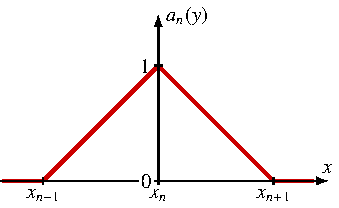
\includegraphics{papers/fem/images/linear_formfkt.pdf}\label{fem:1d:abb:linear:formfkt}}
    \hfill
    \subfloat[Skalierte Formfunktionen mit der zu interpolierenden Funktion $f(x)$]{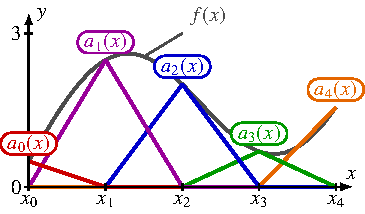
\includegraphics{papers/fem/images/linear_formfkt_skaliert.pdf}\label{fem:1d:abb:linear:skaliert}}

    \subfloat[Gegenüberstellung der interpolierten und der uhrsprünglichen Funktion.]{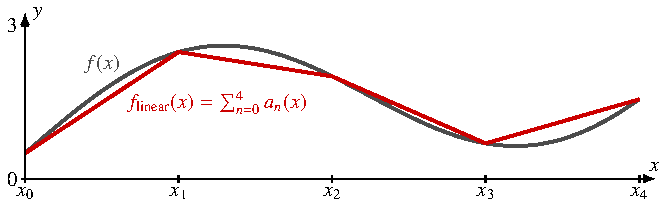
\includegraphics{papers/fem/images/linear_interpoliert.pdf}\label{fem:1d:abb:linear:vergleich}}
    \caption{Lineare Interpolation des Signals $f(x)$.}
    \label{fem:1d:abb:linear}
\end{figure}
     % TODO: Widerholende Formfunktionen und Summe deren als Graphen zeigen
Der lineare Ansatz verwendet die einfachen linearen Funktionen
\begin{equation}
    a(x) = \left\{ \begin{array}{ll}
        1+\frac{x}{\Delta x} & \mbox{für} -\Delta x < x < 0 \\
        1-\frac{x}{\Delta x} & \mbox{für} 0 \leq x < \Delta x \\
        0                    & \mbox{sonst}.
    \end{array} \right.
\end{equation}

Diese Funktionen können mit dem Ansatz 
\begin{equation}
    a(x) = c_1x + c_0 % TODO: Zwei verschiedene a aber keine nicht verwendeten Buchstaben
\end{equation}
und den zu erfüllenden Bedingungen
\begin{equation}
    \begin{array}{ccc}
        a(0) = 1 & \mbox{und} & a(-\Delta x) = a(\Delta x) = 0
    \end{array}
\end{equation}
hergeleitet werden.

\subsubsection{Quadratischer Ansatz}
%
% quadratischer_ansatz.tex
%
% (c) 2024 Flurin Brechbühler
%
\begin{figure}
    \centering
    \subfloat[Formfunktionen des quadratischen Ansatzes]{
        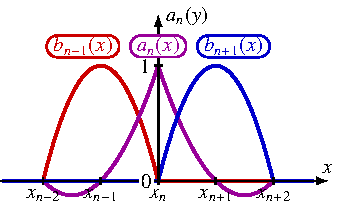
\includegraphics[scale=0.95,valign=t]{papers/fem/images/quadratisch_formfkt.pdf}
        \vphantom{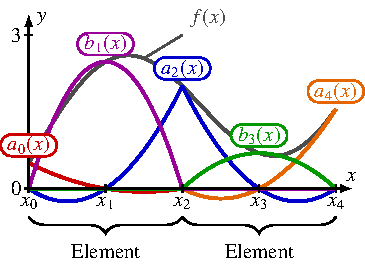
\includegraphics[width=0.45\textwidth,valign=t]{papers/fem/images/quadratisch_formfkt_skaliert.pdf}}
        \label{fem:1d:abb:quadratisch:formfkt}
    }
    \hfill
    \subfloat[Skalierte Formfunktionen mit der zu interpolierenden Funktion $f(x)$]{
        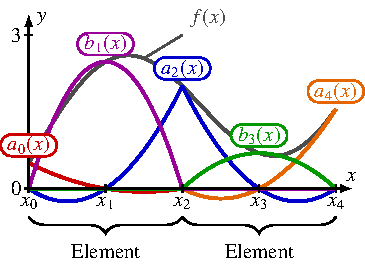
\includegraphics[scale=0.95,valign=t]{papers/fem/images/quadratisch_formfkt_skaliert.pdf}
        \vphantom{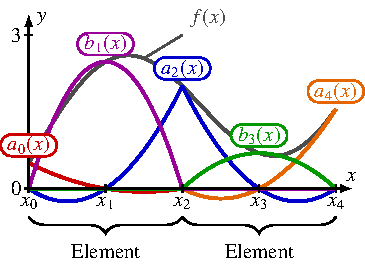
\includegraphics[width=0.45\textwidth,valign=t]{papers/fem/images/quadratisch_formfkt_skaliert.pdf}}
        \label{fem:1d:abb:quadratisch:skaliert}
    }

    \subfloat[Gegenüberstellung der interpolierten und der ursprünglichen Funktion.]{
        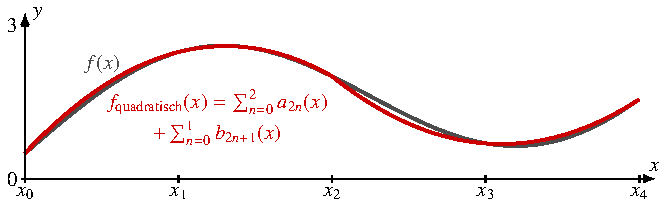
\includegraphics[scale=0.95]{papers/fem/images/quadratisch_interpoliert.pdf}
        \label{fem:1d:abb:quadratisch:vergleich}
    }
    \caption{Quadratische Interpolation des Signals $f(x)$.}
    \label{fem:1d:abb:quadratisch}
\end{figure}
     % TODO: Widerholende Formfunktionen und Summe deren als Graphen zeigen
Der quadratische Ansatz mit den Formfunktionen
\begin{equation}
    a(x) = \left\{ \begin{array}{ll}
        TODO: Formel & \mbox{für} -2 \Delta x < x < 0 \\
        TODO: Formel & \mbox{für} 0 \leq x < 2 \Delta x \\
        0            & \mbox{sonst}
    \end{array} \right.
\end{equation}
für gerade $n$ und
\begin{equation}
    a(x) = \left\{ \begin{array}{ll}
        TODO: Formel & \mbox{für} -\Delta x < x < 0 \\
        TODO: Formel & \mbox{für} 0 \leq x < \Delta x \\
        0            & \mbox{sonst}
    \end{array} \right.
\end{equation}
für ungerade $n$ ist einiges aufwändiger als der lineare Ansatz.

Auch er kann mittels dem Ansatz 
\begin{equation}
    a(x) = c_2x^2 + c_1x + c_0
\end{equation}
und den Bedingungen 
\begin{equation}
    \begin{array}{ccc}
        a(0) = 1 & \mbox{und} & a(-2 \Delta x) = a(-\Delta x) = a(\Delta x) = a(2 \Delta x) = 0
    \end{array}
\end{equation}
für gerade $n$ bzw.
\begin{equation}
    \begin{array}{ccc}
        a(0) = 1 & \mbox{und} & a(-\Delta x) = a(\Delta x) = 0
    \end{array}
\end{equation}
für ungerade $n$ hergeleitet werden.

\subsubsection{Kubischer Ansatz}
%
% linearer_ansatz.tex -- Formfunktionen linearer Ansatz
%
% (c) 2024 Flurin Brechbühler
%
\documentclass[tikz]{standalone}
\usepackage{amsmath}
\usepackage{times}
\usepackage{txfonts}
\usepackage{pgfplots}
\usepackage{csvsimple}

\usetikzlibrary{arrows,intersections,math}
\definecolor{darkred}{rgb}{0.8,0,0}
\definecolor{darkpurple}{rgb}{0.6,0,0.6}
\definecolor{darkblue}{rgb}{0,0,0.8}
\definecolor{darkgreen}{rgb}{0,0.6,0}

\begin{document}
\def\skala{1}

\begin{tikzpicture}[>=latex,thick,scale=\skala]
\begin{scope}

% Plots
	% a_n
\draw[color=darkred,line width=1.4pt] plot[domain=-1.025:-1, scale=4, smooth]
({\x},{0});
\draw[color=darkred,line width=1.4pt] plot[domain=-1:0, scale=4, smooth]
({\x},{(1-2*\x)*(\x+1)^2});
\draw[color=darkred,line width=1.4pt] plot[domain=0:1, scale=4, smooth]
({\x},{(1+2*\x)*(1-\x)^2});
\draw[color=darkred,line width=1.4pt] plot[domain=1:1.025, scale=4, smooth]
({\x},{0});
	% b_n
\draw[color=darkpurple,line width=1.4pt] plot[domain=-1.025:-1, scale=4, smooth]
({\x},{0});
\draw[color=darkpurple,line width=1.4pt] plot[domain=-1:0, scale=4, smooth]
({\x},{\x*(\x+1)^2});
\draw[color=darkpurple,line width=1.4pt] plot[domain=0:1, scale=4, smooth]
({\x},{\x*(1-\x)^2});
\draw[color=darkpurple,line width=1.4pt] plot[domain=1:1.025, scale=4, smooth]
({\x},{0});

% x-Achse
\draw[->] (-4.1,0) -- (4.4,0) coordinate[label={$x$}];
\draw (4,-0.1) -- (4,0.1);
\draw (-4,-0.1) -- (-4,0.1);
\node at (-4,0) [below] {$x_{n-1}$};
\node at ( 0,0) [below] {$x_n$};
\node at ( 4,0) [below] {$x_{n+1}$};

% y-Achse
\draw[->] (0,{-0.1}) -- (0,{4.3})
coordinate[label={right:$y$}];
\node at (-0.1,0) [left, inner sep=1pt, fill=white, rounded corners] {$0$};
\draw (-0.1,4) -- (0.1,4);
\node at (0,4) [left] {$1$};

\end{scope}
\end{tikzpicture}
\end{document}
 % TODO: Widerholende Formfunktionen und Summe deren als Graphen zeigen
Der kubische Ansatz erbringt die Möglichkeit, den Wert der Funktion wie auch den Wert der Ableitung an den Stützstellen frei zu wählen.
Dafür muss der Ansatz etwas erweitert werden:
\begin{equation}
    u(x) \approx \sum{u_n \cdot a_n(x)} \rightarrow u(x) \approx \sum{u_n \cdot a_n(x) + u'_n \cdot b_n(x)}.
\end{equation}

Die Formfunktionen
\begin{equation}
    a(x) = \left\{ \begin{array}{rcl}
        TODO: Formel & \mbox{für} -\Delta x < x < 0 \\
        TODO: Formel & \mbox{für} 0 \leq x < \Delta x \\
        0            & \mbox{sonst}
    \end{array} \right.
\end{equation}
und
\begin{equation}
    b(x) = \left\{ \begin{array}{rcl}
        TODO: Formel & \mbox{für} & -\Delta x < x < 0 \\
        TODO: Formel & \mbox{für} & 0 \leq x < \Delta x \\
        0            & \mbox{sonst}
    \end{array} \right.
\end{equation}
können ebenfalls mit dem Ansatz
\begin{equation}
    a(x) = c_3x^3 + c_2x^2 + c_1x + c_0 \mbox{bzw.} b(x) = c_3x^3 + c_2x^2 + c_1x + c_0
\end{equation}
und den Bedingungen 
\begin{equation}
    \begin{array}{ccc}
        a(0) = 1 & \mbox{und} & a(-\Delta x) = a(\Delta x) = 0
    \end{array}
\end{equation}
und
\begin{equation}
    \begin{array}{ccc}
        b(0) = 1 & \mbox{und} & b(-\Delta x) = b(\Delta x) = 0
    \end{array}
\end{equation}
hergeleitet werden.


\subsection{Lineares Gleichungssystem aufstellen\label{fem:1d:lineares_gleichungssystem}}
Mit den Approximationen 
\begin{align}
    f(x) &\approx \sum_i f_i \cdot a_i(x) \\
    u(x) &\approx \sum_i u_i \cdot a_i(x) \\
    v(x) &\approx \sum_i v_i \cdot a_i(x)
\end{align}
aus der Diskretisierung kann die Schwache Form der Differentialgleichung 
\begin{equation}
    - \int u'(x) \cdot v'(x) \diff x = \int f(x) \cdot v(x) \diff x
\end{equation}
als
\begin{equation}
    - \int \left(\sum_i u_j \cdot a'_j(x)\right) \left(\sum_j v_i \cdot a'_i(x)\right) \diff x 
    = \int \left(\sum_i f_j \cdot a_j(x) \right) \left(\sum_j v_i \cdot a_i(x) \right) \diff x 
    \myforall v_i
\end{equation}
geschrieben werden.
Die Bedingung $\forall v_i$ ist auch erfüllt, wenn die Summe über i sowie die multiplikation mit dem beliebigen Faktor $v_i$ weggelassen wird und die resultierende Gleichung für alle $i$ erfüllt sein muss: % TODO: Proof this... Or argue better
\begin{equation}
    - \int \sum_j u_j \cdot a'_j \cdot a'_i(x) \diff x = \int \sum_j f_j \cdot a_j(x) \cdot a_i(x) \diff x \myforall i
\end{equation}

Dies ermöglicht es, die Summen aus den Integralen zu bringen und die Gleichung als
\begin{equation}
    - \sum_j u_j \int a'_j \cdot a'_i(x) \diff x = \sum_j f_j \int a_j(x) \cdot a_i(x) \diff x \myforall i \label{papers:fem:prinzip1d:finale_gleichung}
\end{equation}
zu schreiben.
Übrig bleibt also, da die Integrale ausgewertet werden können, ein lineares Gleichungssystem mit $N$ Unbekannten $u_j$ und $N$ Gleichungen (eine pro $i$). 


\subsection{Überführung in eine Matrix\label{fem:1d:final_eq}}
Das im vorherigen Schritt erhaltene Gleichungssystem lässt sich sehr gut als Matrizen, bei denen die Zeilen über $i$ und die Spalten über $j$ iterieren, darstellen:
\begin{multline}
    \left(
        \begin{matrix}
            \int a'_1(x) \cdot a'_1 \diff x & \hdots & a'_N(x) \cdot a'_1(x) \diff x \\
            \vdots                          & \ddots & \vdots                        \\
            \int a'_1(x) \cdot a'_N \diff x & \hdots & a'_N(x) \cdot a'_N(x) \diff x \\
        \end{matrix}
    \right)
    \left(
        \begin{matrix}
            u_1 \\
            \vdots \\
            u_N
        \end{matrix}
    \right) \\
    = \\
    \left(
        \begin{matrix}
            \int a_1(x) \cdot a_1 \diff x & \hdots & a_N(x) \cdot a_1(x) \diff x \\
            \vdots                        & \ddots & \vdots                      \\
            \int a_1(x) \cdot a_N \diff x & \hdots & a_N(x) \cdot a_N(x) \diff x \\
        \end{matrix}
    \right)
    \left(
        \begin{matrix}
            f_1 \\
            \vdots \\
            f_N
        \end{matrix}
    \right),
\end{multline}
was kompakt als
\begin{equation}
    \mathbf{M}\vec{f} = -\mathbf{L}\vec{u}
\end{equation}
geschrieben wird.
Auch gängig ist das Zusammenfassen von $\mathbf{M}\vec{f}$ zu $\vec{b}$, was zur Gleichung
\begin{equation}
    \mathbf{L}\vec{u} + \vec{b} = 0
\end{equation}
führt.

Diese Matrizen werden aufgrund des schmalen Trägers der Funktionen $a_n(x)$ (sowie $b_n()$ beim kubischen Ansatz) sehr schwach besetzt sein, da viele der Integralen
\begin{equation}
    \int a_i(x) \cdot a_j \diff x \mbox{ bzw. } \int a'_i(x) \cdot a'_j \diff x 
\end{equation}
Null sein werden.
Von Null verschieden sind nur die Einträge, deren zugehörige Datenpunkte nebeneinander liegen.
Zudem sind sie symmetrisch und positiv definit, da es keine Rolle spielt in welcher Reihenfolge man die Testfunktionen multipliziert.

\subsubsection{Kubischer Ansatz}
Auch hier verlangt der kubische Ansatz mit seinen zwei Funktionen pro Datenpunkt eine leichte Anpassung: 
\begin{itemize}
    \item Die Vektoren $\vec{b}$ und $\vec{f}$ werden für die gleiche Menge Datenpunkte doppelt so viele Elemente enthalten.
          Dies aus dem Grund, dass für jeden Wert $u_i$ ein zweiter Wert $u'_i$ dazukommt.
    \item Die Matrix $\mathbf{L}$ wird zwangsweise doppelt so viele Zeilen und Spalten enthalten müssen, um mit den neuen Werten rechnen zu können. % TODO: Diese Begrüngung ist noch nicht ganz zufriedenstellend.
\end{itemize}


\subsection{Codieren der Anfangsbedingungen}
TODO: Erklären, wie Anfangsbedingungen codiert werden können


\subsection{Invertieren der Matrix\label{fem:1d:invertieren_matrix}}
Zur Lösung der Poisson gleichung muss nun also nur noch die Matrix $\mathbf{L}$ invertiert werden.
Das Resultat in Form des Spaltenvektors $\vec{u}$, enthaltend der Stützstellen der Lösungsfunktion, lässt sich dann als
\begin{equation}
    \vec{u} = - \mathbf{L}^{-1}\mathbf{M}\vec{f} = - \mathbf{L}^{-1}\vec{b}
\end{equation}
berechnen.

Zum Invertieren der Matrix gibt es optimierte Zerlegungsalgorytmen wie SuperLU, Choldmod oder Mumps, die die schwache Besetzung der Matrizen ausnützen, um diese effizient zu zerlegen.
Nach dem Zerlegen ist das Invertieren stark vereinfacht.
Weiter bieten sich iterative Vorgehen wie die Methode des konjugierten Gradienten oder GMRES an.
Auch diese können aus der schwachen Besetzung der Matrix nutzen ziehen.

TODO: properly research and cite this. Research notes for now.
